\section{Lecture 17: FIR Filter Design (Chebyshev)}

In the previous lecture, we spoke about FIR filter design using the
least-squares approximation; we specified a number of points in
a desired filter's amplitude response and created a filter which
interpolated between these points. This scheme can be problematic
since it doesn't allow us to specify the form of the filter
between the interpolated points; the ripple is something that we
can't really control. The focus of this lecture is to provide a
scheme whereby the created filter doesn't deviate by more than
some specified amount in the pass-band and stop-band.\\
%
To this end, we introduce a different error function from the
least-squares version. Define the Chebyshev cost function as
%
\begin{displaymath}
  \min E = \max_{\omega\in[0,\pi)} \lvert A(\omega) - A_\mathrm{des}(\omega)\rvert \,,
\end{displaymath}
%
i.e. over the range $[0,\pi)$, the filter error is defined as the
maximum deviation between the desired filter and the filter we've
created. Filters that are optimal with respect to this criterion
are called \textbf{Equiripple}. An equiripple filter is presented
in Figure \ref{fig::lecture_17_equiripple}. We can define some
tolerance in the ripple in the
passband and stopband, and as long as the filter length is
compatible with these specifications, we can drive the filter
response to being as desired.\\
%
\begin{figure}[!htb]
  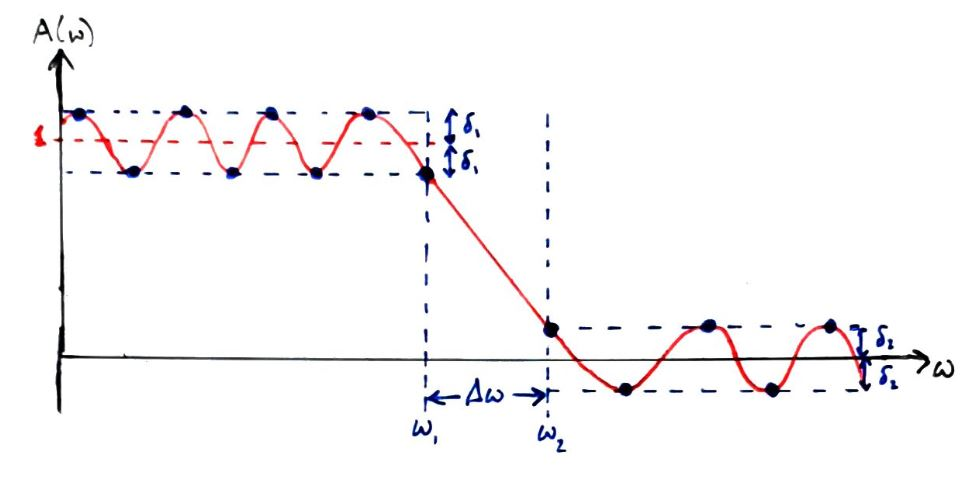
\includegraphics[width=\textwidth]{images/lecture_17_equiripple.JPG}
  \caption{
  }
  \label{fig::lecture_17_equiripple}
\end{figure}
%
An acceptable frequency response has the following characteristics:
%
\begin{enumerate}
\item Linear phase FIR filters (since the filter is real, anti/symmetric
  and only introduce delays into the output).
\item Some width, $\Delta\omega$, of the transition band.
\item Deviation from $1$ in the pass-band of $\pm\delta_1$.
\item Deviation from 0$0$ in the stop-band of $\pm\delta_2$.
\end{enumerate}

Before progressing, it is worth introducing the Chebyshev polynomials
of the first kind,
%
\begin{displaymath}
  T_n(x) = \cos\left(n\cos^{-1}x\right) \quad\Longleftrightarrow\quad
  T_n(\cos \theta) = \cos n\theta \,.
\end{displaymath}
%
From the double-angle formulae, we know that
%
\begin{displaymath}
  \cos 0\theta = 1, \quad \cos 1\theta = \cos\theta, \quad \cos 2\theta = 2\cos^2\theta + 1, \hdots \,,
\end{displaymath}
%
allowing us to conclude that
%
\begin{displaymath}
  T_0(x) = 1, \quad T_1(x) = x, \quad T_2(x) = 2x^2 + 1, \hdots \,,
\end{displaymath}
%
i.e. $\cos(n\theta)$ is some $n\th$ order polynomial in $x = \cos\theta$.
As such, for some generic sum of cosines,
%
\begin{displaymath}
  S(x) = \sum_{n=0}^{N-1} c_n\cos(n\theta)
  = \sum_{n=0}^{N-1}c_n\cos(n\cos^{-1}x)
  = \sum_{n=0}^{N-1} d_nT_n(x) \,.
\end{displaymath}
%
This equivalence between cosines and polynomials (and sums thereof) presents
a change of variables that we'll find useful later in this lecture.

\subsection{The Approximation Problem}
%
Previously, we showed that the amplitude response of a Type I linear
phase filter can be written as some linear combination of cosines 
%
\begin{displaymath}
  A(\omega) = \sum_{k=0}^{r-1}c_k \cos(\omega k) \,,
\end{displaymath}
%
where $r=\frac{N+1}{2}$. Our aim now is to minimise the Chebyshev cost
function subject to the constraint that our amplitude response be
given by the above linear combination of cosines. The
\textbf{approximation problem} can then be written as, given
%
\begin{enumerate}
\item A set of frequency bands in $[0,\pi]$.
\item A desired real-valued $A_\mathrm{des}(\omega)$ in these bands.
\item A positive weight function, $W(\omega)$.
\item The form $A(\omega) = \sum_{k=0}^{r-1}c_k \cos(\omega k)$
\end{enumerate}
%
find $\{c_k\}$. To do this, we need to solve using the
\textbf{alternation theorem}: if $A(\omega)$ is a sum of $r$ cosines,
then a necessary and sufficient condition for $A(\omega)$ to be the
unique best-weighted Chebyshev (equiripple) approximation to
$A_\mathrm{des}(\omega)$ on the given bands is that
%
\begin{displaymath}
  E(\omega) = W(\omega)\lvert A(\omega) - A_\mathrm{des}(\omega) \rvert
\end{displaymath}
%
must exhibit at least $r+1$ extremal frequencies in the given bands,
where extremal frequencies are some $\{\omega_i\}$ such that
%
\begin{displaymath}
  E(\omega_i) = \max E(\omega) \quad\mathrm{and}\quad E(\omega_i) = -E(\omega_{i+1}) \,.
\end{displaymath}
%
This is depicted in Figure \ref{fig::lecture_17_equiripple}
for a length-25 FIR filter (i.e. $r+1 = \frac{N+1}{2} = 13$. If we
recognise that there are $r+1$ extremal frequencies in a filter, then
we can say that the filter is optimal with respect to the Chebyshev
cost function.

\subsection{The Remez Exchange Algorithm}
%
The Remez exchange algorithm is an iterative process for finding
an optimal equiripple filter by first guessing its extremal
frequencies, and iterating until our constraints are met. Consider
our cost function,
%
\begin{displaymath}
  E(\omega) = A_\mathrm{des}(\omega) - \sum_{k=0}^{r-1}c_k\cos(\omega k) \,,
\end{displaymath}
%
which can be made to take on the values $\pm\delta$ for any given set
of frequency bands $\{\omega_1,\hdots,\omega_{r+1}\}$, i.e.
%
\begin{equation}\label{eq::remez}
  A_\mathrm{des}(\omega_m) = \sum_{k=0}^{r-1}\cos(\omega_m k) + (-1)^m\delta \,,
\end{equation}
%
for all $i = 1, \hdots, r+1$. There exists a unique solution to this
for the combination of $\{c_k\}$ and $\delta$.\\
%
Consider an initial set of guesses for the extremal frequencies,
$T_0 = \{\omega_1,\hdots,\omega_{r+1}\}$. The Remez Exchange Algorithm
then follows:
%
\begin{enumerate}
\item Solve the linear equations in Equation \ref{eq::remez}, the solution of
  which has an error that oscillates with amplitude $\delta_k$ on the
  extremal frequencies $T_k$.
\item Interpolate to find the frequency response on all of $[0,\pi]$.
\item Search $[0,\pi]$ to see if and where the magnitude of the error
  exceeds $\delta_k$.
\item If the maximum error is equal to $\delta_k$, we are done. Otherwise,
  take the $r+1$ maximal frequencies in this new frequency response as
  $T_{k+1}$ and return to the first step.
\end{enumerate}
%
\begin{exmp}
  Try to approximate $A_\mathrm{des}(\omega) = x^2$ by $A(\omega) = d_0 + d_1 x$
  over $[0,1]$ using the Chebyshev cost function. In other words, solve
  %
  \begin{displaymath}
    \min_{d_1,d_2}E = \max_{\omega\in[0,1]}\lvert x^2 - (d_0 + d_1 x)\rvert \,.
  \end{displaymath}
  %
  Since we have a second order polynomial in $x$, we are looking for 3 extremal
  frequencies. To begin the Remez exchange algorithm, begin by guessing
  $T_0 = \{1/4, 1/2, 1\}$, the points at which we make the error oscillate, i.e.
  %
  \begin{displaymath}
    x_k^2 = d_0 + d_1x_k + (-1)^k\delta \,,
  \end{displaymath}
  %
  where $d_0, d_1, \delta$ are unknown. This can be formulated as three equations
  in three unknowns,
  %
  \begin{displaymath}
    \left[\begin{array}{ccc}
        1 & x_0 & (-1)^0 \\
        1 & x_1 & (-1)^1 \\
        1 & x_2 & (-1)^2
      \end{array}\right]
    \left[\begin{array}{c}d_0 \\ d_1 \\ \delta \end{array}\right]
    = \left[\begin{array}{c}x_0^2 \\ x_1^2 \\ x_2^2\end{array}\right]
  \quad\longrightarrow\quad
    \left[\begin{array}{ccc}
        1 & \frac{1}{4} & 1 \\
        1 & \frac{1}{2} & -1 \\
        1 & 1 & 1
      \end{array}\right]
    \left[\begin{array}{c}d_0 \\ d_1 \\ \delta \end{array}\right]
    = \left[\begin{array}{c}\frac{1}{16} \\ \frac{1}{4} \\ 1\end{array}\right]  
  \end{displaymath} \,,
  %
  which when solved yields $d_0 = -5/16, d_1 = 5/4, \delta = 1/16$. The
  cost function for this is plotted in Figure
  \ref{fig::lecture_17_remez_iteration}. We see that at the
  points $T_0$, we indeed have an error of $\delta = 1/16$, but this is
  by no means the smallest error on the domain $[0,\pi]$; rather,
  $\max_{[0,\pi]}E(x) = E(0) = 5/16$, and consequently we need to iterate
  the Remez exchange, this time using $T_1 = \{0, 5/8, 1\}$, those values of
  $x$ where $E(x)$ is extremal,
  %
  \begin{displaymath}
    \left[\begin{array}{ccc}
        1 & 0 & 1 \\
        1 & \frac{5}{8} & -1 \\
        1 & 1 & 1
      \end{array}\right]
    \left[\begin{array}{c}d_0 \\ d_1 \\ \delta \end{array}\right]
    = \left[\begin{array}{c}0 \\ \frac{25}{64} \\ 1\end{array}\right] \,,  
  \end{displaymath}
  %
  which when solved yields $d_0 = -15/128, d_1 =1, \delta =15/128$. The
  cost function for this is plotted in Figure \ref{fig::lecture_17_remez_iteration}.
  As before, we see
  that $\max_{[0,\pi]}E(x) = E(1/2) = 17/128$, which is greater than
  $\delta$, and consequently we set $T_2 = \{0, 1/2, 1\}$,
  %
  \begin{displaymath}
    \left[\begin{array}{ccc}
        1 & 0 & 1 \\
        1 & \frac{1}{2} & -1 \\
        1 & 1 & 1
      \end{array}\right]
    \left[\begin{array}{c}d_0 \\ d_1 \\ \delta \end{array}\right]
    = \left[\begin{array}{c}0 \\ \frac{1}{4} \\ 1\end{array}\right] \,,  
  \end{displaymath}
  %
  which when solved yields $d_0 = -1/8, d_1 = 1, \delta = 1/8$, the cost function of
  which is plotted in Figure \ref{fig::lecture_17_remez_iteration}. Now we see that
  the extremal frequencies
  are indeed $T_2$, and the Remez exchange algorithm has converged. The best
  approximation is then $A(x) = d_0 + d_1 x = - \frac{1}{8} + x$.
  %
  \begin{figure}[!htb]
    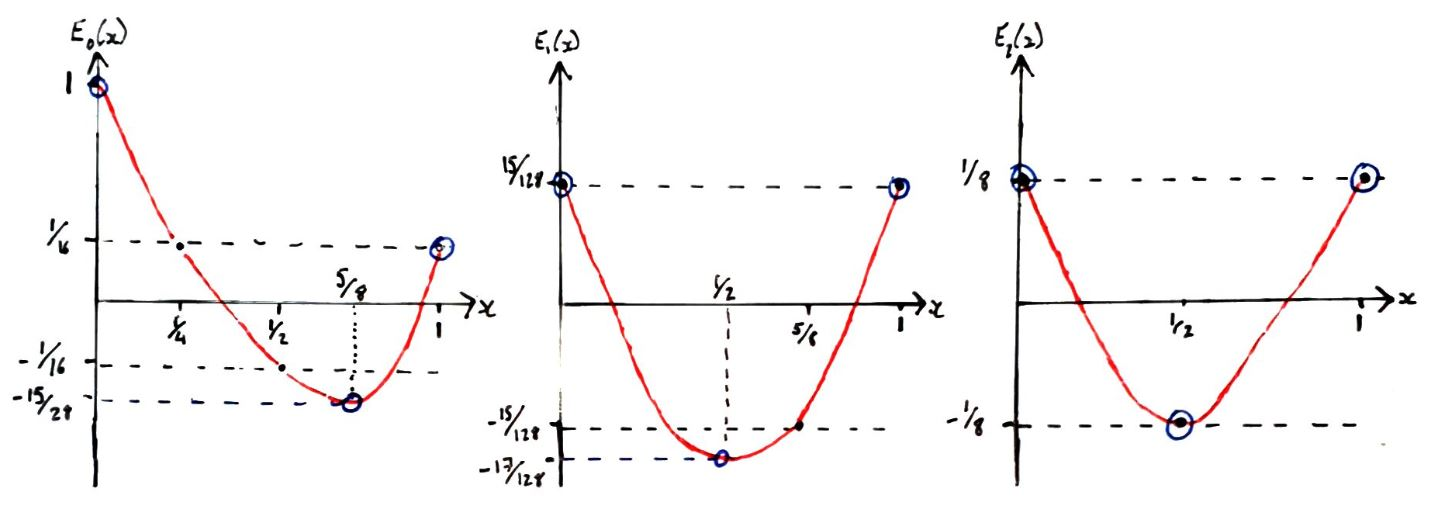
\includegraphics[width=\textwidth]{images/lecture_17_remez_iteration.JPG}
    \caption{
    }
    \label{fig::lecture_17_remez_iteration}
  \end{figure}

\end{exmp}
%
The Remez Exchange Algorithm always converges to an equiripple approximation,
\textbf{but} it may not have the desired pass-band and stop-band characteristics for
a given filter order. For instance, we can't make the ripple arbitrarily small
given only 3 filter taps; we can only do so well with a finite number of
parameters.\\
%
To characterise an equiripple filter, one needs to know the filter length, $N$,
its pass-band and stop-band edges, $\omega_1$ and $\omega_2$, and the pass-band
and stop-band deviations, $\delta_1$ and $\delta_2$. Given that the filter of
length $N$ might not be able to converge to this specification, we can invoke a
heuristic, to calculate the $N$ which satisfies these criteria,
%
\begin{displaymath}
  N \approx \frac{-20 \log_10\sqrt{\delta_1\delta_2} - 13}{14.6(\omega_2 - \omega_1)} + 1 \,.
\end{displaymath}
%
As the pass-band and stop-band are brought closer together, $\omega_2 - \omega_1$
becomes smaller and $N$ increases as we might expect. Similarly if we want
the deviation to increase, $\delta_1\delta_2$ increases and the
filter also increases. Signal processing toolboxes obviously offer
a means to design filters using the Remez Exchange Algorithm,
the Parks-McClellan algorithm is one such variant of an iterative
means to find the optimal Chebyshev FIR filter given a parameterisation.
%
\begin{exmp}
  Consider a low-pass filter where $N=11$ where $\omega_1 = 0.3\pi$ and
  $\omega_2 = 0.5\pi$. The code given in \texttt{scripts/lecture\_17\_remez.py}
  QQ. Its output is visualised in Figure \ref{fig::lecture_17_remez_example}.
  %
  \begin{figure}[!htb]
    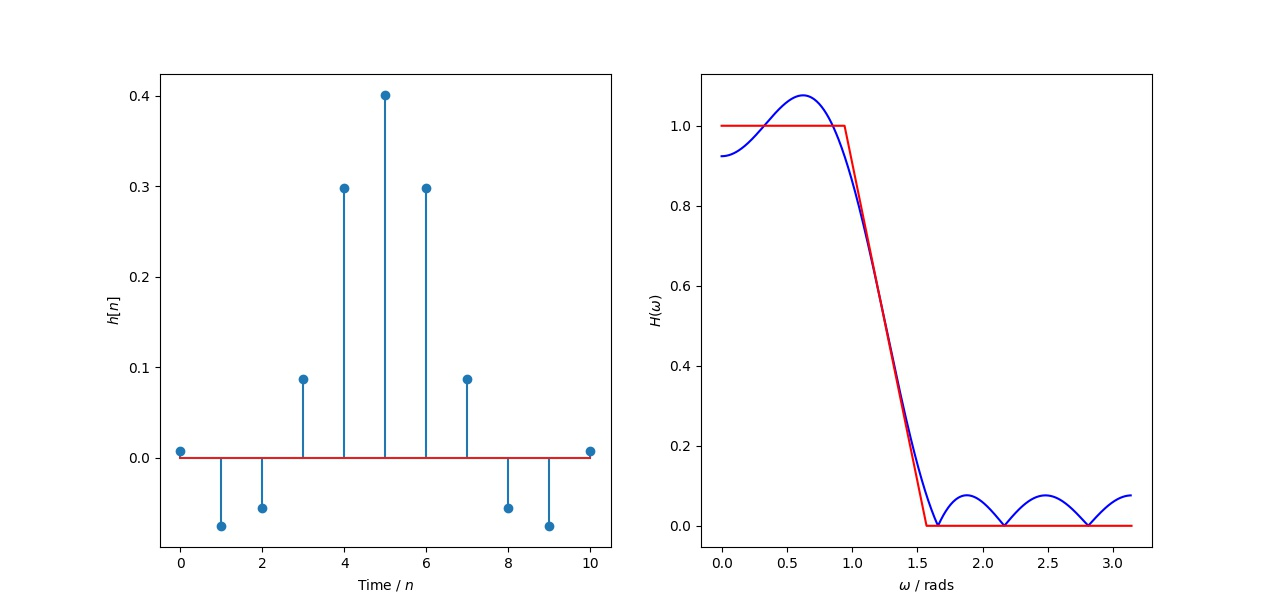
\includegraphics[width=\textwidth]{images/lecture_17_remez_example.JPG}
    \caption{
    }
    \label{fig::lecture_17_remez_example}
  \end{figure}
  %
\end{exmp}

\subsection{FIR Advantages and Disadvantages}
%
The advantages of using an FIR filter include:
%
\begin{enumerate}
\item We can achieve exactly linear phase filters; there's always
  some midpoint in the filter about which it is symmetry. This is
  not the case with an IIR filter since there is no midpoint, which
  consequently leads to some kind of distortion.
\item Easy and efficient implementation.
\item Easily designed with linear methods.
\item Filters are always stable since there are no poles, by definition.
\end{enumerate}
%
The disadvantages of using an FIR filter include:
%
\begin{enumerate}
\item May require a large number of taps, $N$, in the filter to achieve good
  approximations to some frequency responses (see the heuristic in
  the previous section). This is problematic for real-time processing since
  it's undesirable to introduce a large delay, $N$ between input and
  output.
\item May need many operations per output, and may need to store
  a lot of coefficients, which is constraining for some embedded systems.
\end{enumerate}
